\documentclass[xcolor=pdftex,dvipsnames,table,mathserif,aspectratio=169]{beamer}
\usetheme{metropolis}

\usepackage[english]{babel}
\usepackage{pgf,pgfarrows,pgfnodes,pgfautomata,pgfheaps}
\usepackage{amsmath,amssymb,setspace,centernot}
\usepackage[latin1]{inputenc}
\usepackage[T1]{fontenc}
\usepackage{relsize}
\usepackage{pdfpages}
\usepackage[absolute,overlay]{textpos} 

\newenvironment{reference}[2]{% 
  \begin{textblock*}{\textwidth}(#1,#2) 
      \footnotesize\it\bgroup\color{red!50!black}}{\egroup\end{textblock*}} 

\DeclareMathSizes{10}{10}{6}{6} 
\AtBeginSection[]{
  \begin{frame}
  \vfill
  \centering
  \begin{beamercolorbox}[sep=8pt,center,shadow=true,rounded=true]{title}
    \usebeamerfont{title}\insertsectionhead\par%
  \end{beamercolorbox}
  \vfill
  \end{frame}
}


\DeclareMathOperator*{\argmax}{arg\,max}
\DeclareMathOperator*{\argmin}{arg\,min}

\newcommand{\norm}[1]{\left\lVert#1\right\rVert}
\newcommand{\X}{\mathtt{X}}
\newcommand{\Y}{\mathtt{Y}}

%\newcommand{\R}{\mathbb{R}}
%\newcommand{\E}{\mathbb{E}}
%\newcommand{\V}{\mathbb{V}}
\newcommand{\p}{\mathbb{P}}
\newcommand*\df{\mathop{}\!\mathrm{d}}
\newcommand{\del}{\partial}

\begin{document}
\title{Instruments and Identification }
\author{Chris Conlon}
\institute{Grad IO}
\date{\today}

\frame{\titlepage}

\begin{frame}{Parametric Identifcation}
\begin{itemize}
\item Once we have $D_{jt}^{-1}(\mathcal{S}_t,\widetilde{\theta}_2)\equiv \delta_{jt}(\theta_2)$ identification of linear parameters is pretty straightforward
\begin{eqnarray*}
D_{jt}^{-1}(\mathcal{S}_t,\widetilde{\theta}_2) = x_{jt} \beta -  \alpha \cdot \alert{ p_{jt}} + \xi_j + \xi_t + \Delta \xi_{jt}
\end{eqnarray*}
\item This is either basic linear IV or panel linear IV and we need instruments for $p_{jt}$
\item The $\widetilde{\theta}_2$ parameters governing the change of variables require \alert{nonlinear IV}
\item Remember $\theta_2 =  [\widetilde{\theta}_2, \alpha]$.
\end{itemize}
\end{frame}

\begin{frame}{Exclusion Restrictions}
\begin{eqnarray*}
    \delta_{jt}(\mathcal{S}_t,\widetilde{\theta}_2) &=&  h_d\left(x_{jt}, \alert{v_{jt}}; \theta_1 \right)  - \alpha p_{jt} + \xi_{jt}\\
    f(p_{jt} - \eta_{jt}(\theta_2,\mathbf{p},\mathbf{s})) &=&   h_d\left(x_{jt},\alert{w_{jt}};\theta_3 \right)+\omega_{jt}
\end{eqnarray*}
The first place to look for exclusion restrictions/instruments:
\begin{itemize}
\item Something in another equation!
\item $v_j$ shifts demand but not supply
\item $w_j$ shifts supply but not demand
\item If it doesn't shift either is it really relevant?
\end{itemize}
\end{frame}

\begin{frame}{Markup Shifters}
The equilibrium markup is a function of \alert{everything!} $\eta_{jt}(\mathbf{p},\mathbf{s},\xi_t,\omega_t,x_{t},w_{t},v_t,\theta_2)$:
\begin{itemize}
\item It is literally \alert{endogenous} (depends on error terms)!
\item But lots of potential instruments beyond \alert{excluded} $v_t$ or $w_t$.
\item Also $v_{-j}$ and $w_{-j}$ and $x_{-j}$ (these don't depend on $\xi_{jt},\omega_{jt}$)
\item Not $p_{-j}$ or $\xi_{-j}$, (these depend on $\xi_{jt},\omega_{jt}$).
\item The idea is that these instruments shift or rotate the \alert{marginal revenue curve}.
\item What is a good choice of $f(x_{-j})$? etc.
\end{itemize}
\end{frame}

\begin{frame}{What are we instrumenting for?}
\begin{itemize}
\item Recall the nested logit, where there are two separate endogeneity problems
\begin{itemize}
\item Endogenous \alert{markups} $\eta_{jt}$ (link S+D)
\item \alert{Nonlinear characteristics} $\sigma$ on $\ln s_{j|gt}$ this is the other one.
\end{itemize}
\item Nonlinear parameters $\widetilde{\theta_2}$.
\begin{itemize}
\item Consider increasing the price of $j$ and measuring substitution to other products $k,k'$ etc.
\item If sales of $k$ increase with $p_j$ and $(x_j^{(1)},x_k^{(1)})$ are similar then we increase the $\sigma$ that corresponds to $x^{(1)}$.
\item Price is the most obvious to vary, but sometimes this works for other characteristics (like distance).
\item Alternative: vary the set of products available to consumers by adding or removing an option. In which dimension are close substitutes ``more similar''.
\end{itemize}
\end{itemize}
\end{frame}






\begin{frame}{Instruments}
\begin{itemize}
\item We are doing nonlinear GMM: Start with $E[\xi_{jt} | x_{jt}, w_{jt}]=0$ use $E[\xi_{jt}' Z_{jt}^D]=0$ with $Z_{jt}^D=[x_{jt},\,  z_{jt}]$.
\begin{itemize}
\item In practice this means that for valid instruments $(x,w)$ any function $f(x,w)$ is also a valid instrument $E[ \xi_{jt} f(x_{jt},w_{jt})]=0$.
\item We can use $x, x^2, x^3,\ldots$ or interactions $x \cdot w, x^2 \cdot w^2, \ldots$.
\item What is a reasonable choice of $f(\cdot)$?
\item Where does $w$ come from?
\end{itemize}
\end{itemize}
\end{frame}


\begin{frame}{BLP Instruments}
\begin{itemize}
\item Common choices are average characteristics of other products in the same market $f(x_{-j,t})$. \alert{BLP instruments}
\begin{itemize}
\item Same firm $z_{1jt} = \overline{x}_{-j_f,t} = \frac{1}{\left\vert{F_j}\right\vert}  \sum_{k \in \mathcal{F}_j} x_{kt} - \frac{1}{\left\vert{F_j}\right\vert} x_{jt}$.
\item Other firms $z_{2jt}=\overline{x}_{\cdot t} - \overline{x}_{-j_f,t} - \frac{1}{J} x_{jt}$.
\item Plus regressors $(1, x_{jt})$.
\item Plus higher order interactions 
\end{itemize}
\item Technically linearly independent for large (finite) $J$, but becoming highly correlated.
\begin{itemize}
\item Can still exploit variation in number of products per market or number of products per firm.
\end{itemize}
\item Correlated moments $\rightarrow$ ``many instruments''.
\begin{itemize}
\item May be inclined to ``fix'' correlation in instrument matrix directly.
\end{itemize}
\end{itemize}
\end{frame}


\begin{frame}{Armstrong (2016): Weak Instruments?}
Consider the limit as $J \rightarrow \infty$
\begin{eqnarray*}
\frac{s_{jt}(\mathbf{p_t})}{\left|\frac{\partial s_{jt}(\mathbf{p_t})}{\partial p_{jt}}\right|} = \frac{1}{\alpha} \frac{1}{1-s_{jt}} \rightarrow \frac{1}{\alpha}
\end{eqnarray*}
\begin{itemize}
\item Hard to use markup shifting instruments to instrument for a constant.
\item How close to the constant do we get in practice?
\item Average of $x_{-j}$ seems like an especially poor choice. Why?
\item Shows there may still be some power in: products per market, products per firm.
\item Convergence to constant extends to mixed logits (see Gabaix and Laibson 2004).
\item Suggests that you really need cost shifters.
\end{itemize}
\end{frame}

\begin{frame}{Differentiation Instruments: Gandhi Houde (2019)}
\small
\begin{itemize}
\item Also need instruments for the random coefficient parameters $\widetilde{\theta}_2$.
\item Instead of average of other characteristics $f(x) = \frac{1}{J-1} \sum_{k \neq j} x_k$, can transform as distance to $x_j$.
\begin{eqnarray*}
d_{jkt} =  x_{kt} - x_{jt}  
\end{eqnarray*}
\item And use this transformed to construct two kinds of IV (Squared distance, and count of local competitors)
\begin{eqnarray*}
z_{jt}^{\text{quad}} =& \sum_{k  \in F}  d_{jkt}^2,  \quad &\sum_{k \notin F}  d_{jkt}^2 \\
z_{jt}^{\text{local}} =& \sum_{k \in F}  I[d_{jkt} < c]   \quad &\sum_{k \notin F}   I[d_{jkt} < c]
\end{eqnarray*}
\item They choose $c$ to correspond to one standard deviation of $x$ across markets.
\end{itemize}
\end{frame}




\begin{frame}{Optimal Instruments (Chamberlain 1987)}
Chamberlain (1987) asks how can we choose $f(z_i)$ to obtain the semi-parametric efficiency bound with conditional moment restrictions:
\begin{align*}
E[g(z_i,\theta) | z_i]=0 \Rightarrow E[g(z_i,\theta) \cdot f(z_i) ]=0 
\end{align*}
Recall that the asymptotic GMM variance depends on $(D'\, \Omega^{-1} D\,)$

The answer is to choose instruments related to the (expected) Jacobian of moment conditions w.r.t $\theta$. The true Jacobian at $\theta_0$ is \alert{infeasible}:
\begin{align*}
D=E\left[\frac{\partial g(z_i,\theta)}{\partial \theta} | z_i \right]
\end{align*}
%Dominguez and Lobato (2004) point out we can get unlucky and choose an $f(z_i)$ such that $\theta$ is no longer identified(!)
\end{frame}


\begin{frame}{Optimal Instruments (Chamberlain 1987)}
Consider the simplest IV problem:
\begin{align*}
y_i &= \beta x_i + \gamma v_i + u_i \quad \text{ with } \quad E[u_i | v_i, z_i] =0 \\
u_i &= \left(y_i - \beta x_i - \gamma v_i \right) \\
g(x_i,v_i,z_i) &= \left(y_i - \beta x_i - \gamma v_i \right) \cdot [v_i,\, z_i]
 \end{align*}
 Which gives:
\begin{align*}
E\left[\frac{\partial g(x_i,v_i, z_i,\theta)}{\partial \gamma} \mid v_i, z_i \right] &= v_i\\
E\left[\frac{\partial g(x_i,v_i, z_i,\theta)}{\partial \beta} \mid v_i, z_i \right] &=E\left[x_i \mid v_i, z_i \right]
\end{align*}
We can't just use $x_i$ (bc endogenous!), but you can also see where 2SLS comes from...
\end{frame}



\begin{frame}{Optimal IV: BLP}
Recall the GMM moment conditions are given by $E[\xi_{jt} | Z_{jt}^D]=0$ and $E[\omega_{jt} | Z_{jt}^S]=0$ and the asymptotic GMM variance depends on $(D'\, \Omega^{-1} D\,)$ where the expressions are given below:
\begin{align*}
    D=E\left[
    \left(\frac{\partial \xi_{jt}}{\partial \theta}, \,
    \frac{\partial \omega_{jt}}{\partial \theta} \right)
| \mathbf{Z_t} \right], \quad 
\Omega = E\left[
\begin{pmatrix}
    \xi_{jt} \\
    \omega_{jt}
\end{pmatrix}
\begin{pmatrix}
    \xi_{jt}\, \,
    \omega_{jt}
\end{pmatrix}
| \mathbf{Z_t} \right].
\end{align*}
Chamberlain (1987) showed that the approximation to the optimal instruments are given by the expected Jacobian contribution for each observation $(j,t)$: $E[D_{jt}(\mathbf{Z_t}) \Omega_{jt}^{-1} | \mathbf{Z_t}]$.
\end{frame}

\begin{frame}{Optimal Instruments (Newey 1990)}
From previous slide, nothing says that $E\left[x_i \mid v_i, z_i \right]$ needs to be \alert{linear}!
\begin{itemize}
\item Since any $f(x,z)$ satisfies our orthogonality condition, we can try to choose $f(x,z)$ as a \alert{basis} to approximate optimal instruments.
\item Why? Well affine tranformations of instruments are still valid, and we span the same vector space!
\item We are essentially relying on a non-parametric regression that we never run (but could!)
\begin{itemize}
\item This is challenging in practice -- and in fact suffers from a curse of dimensionality.
\item This is frequently given as a rationale behind higher order $x$'s.
\item When the dimension of $x$ is low -- this may still be feasible. ($K \leq 3)$.
\item But recent improvements in sieves, LASSO, non-parametric regression are encouraging.
\end{itemize}
\end{itemize}
\end{frame}




\begin{frame}{Optimal Instruments (see Conlon Gortmaker 2020)}
\noindent BLP 1999 tells us the (Chamberlain 1987) optimal instruments for this supply-demand system of $G\Omega^{-1}$ where for a given observation $n$, we need to compute $E[\frac{\partial \xi_{jt}}{\partial \theta} | x, v, w]$ and $E[\frac{\partial \omega_{jt}}{\partial \theta} | x, v, w]$

\begin{align*}
    D_{jt} \equiv \underbrace{
        \begin{bmatrix}
            \frac{\partial \xi_{jt}}{\partial \beta}
            & \frac{\partial \omega_{jt}}{\partial \beta} \\
            \frac{\partial \xi_{jt}}{\partial \alpha}
            & \frac{\partial \omega_{jt}}{\partial \alpha} \\
            \frac{\partial \xi_{jt}}{\partial \widetilde{\theta}_2}
            & \frac{\partial \omega_{jt}}{\partial \widetilde{\theta}_2} \\
            \frac{\partial \xi_{jt}}{\partial \gamma} 
            & \frac{\partial \omega_{jt}}{\partial \gamma} 
        \end{bmatrix}
    }_{(K_1 + K_2 + K_3)\times 2}
    = 
    \begin{bmatrix}
        -x_{jt} & 0 \\
        -v_{jt} & 0 \\
        \frac{\partial \xi_{jt}}{\partial \alpha}  
        &  \frac{\partial \omega_{jt}}{\partial \alpha}\\
        \frac{\partial \xi_{jt}}{\partial \widetilde{\theta}_2} 
        & \frac{\partial \omega_{jt}}{\partial \widetilde{\theta}_2} \\
        0 & -x_{jt} \\
        0 & -w_{jt}
    \end{bmatrix}
    , \quad \Omega_t \equiv 
    \underbrace{
        \begin{bmatrix}
        \sigma^2_{\xi_t} & \sigma_{\xi_t \omega_t}\\
        \sigma_{\xi_t \omega_t} & \sigma^2_{\omega_t}
    \end{bmatrix}
    }_{2 \times 2}.
\end{align*}
\end{frame}


\begin{frame}{Optimal Instruments: (see Conlon Gortmaker 2020) }
\noindent I replace co-linear elements with zeros using $\odot \Theta$
\begin{align*}
    (D_{jt} \Omega_t^{-1} ) \odot \Theta =  \frac{1}{\sigma_\xi^2 \sigma_\omega^2 - \sigma_{\xi \omega}^2} \cdot 
    \begin{bmatrix}
        -\sigma_\omega^2 x_{jt} & 0  \\
        -\sigma_\omega^2 v_{jt} & \sigma_{\xi \omega} v_{jt} \\
        \sigma_\omega^2 \frac{\partial \xi_{jt}}{\partial \alpha} - 
        \sigma_{\xi\omega}\frac{\partial \omega_{jt}}{\partial \alpha} 
        & \sigma_{\xi}^2 \frac{\partial \omega_{jt}}{\partial \alpha}  - 
        \sigma_{\xi\omega}\frac{\partial \xi_{jt}}{\partial \alpha}  \\
        \sigma_\omega^2 \frac{\partial \xi_{jt}}{\partial \widetilde{\theta}_2}  -
        \sigma_{\xi\omega}\frac{\partial \omega_{jt}}{\partial \widetilde{\theta}_2} 
        & \sigma_{\xi}^2 \frac{\partial \omega_{jt}}{\partial \widetilde{\theta}_2} - 
        \sigma_{\xi\omega}\frac{\partial \xi_{jt}}{\partial \widetilde{\theta}_2}\\
        0 &  -\sigma_{\xi}^2 x_{jt} \\
        \sigma_{\xi\omega} w_{jt} & -\sigma_{\xi}^2 w_{jt}
    \end{bmatrix}
    .
\end{align*}
\noindent Now we can partition our instrument set by column into ``demand'' and ``supply'': 
\begin{align*}
    Z_{jt}^{\textit{Opt},D} \equiv \underbrace{E[(D_{jt}(Z_t) \Omega_t^{-1} \odot \Theta)_{\cdot 1} | Z_t]}_{K_1 + K_2 + (K_3 - K_x)}, \quad Z_{jt}^{\textit{Opt},S} \equiv \underbrace{E[(D_{jt}(Z_t)\Omega_t^{-1} \odot \Theta)_{\cdot 2} | Z_t]}_{K_2 + K_3+ (K_1 - K_x)}.
\end{align*}
\end{frame}


\begin{frame}{Aside: What does Supply tell us about Demand?}
\begin{align*}
& \textbf{Demand} & \textbf{Supply} \\
\del \alpha:& 
        \sigma_\omega^2 \frac{\partial \xi_{jt}}{\partial \alpha} - 
        \sigma_{\xi\omega}\frac{\partial \omega_{jt}}{\partial \alpha} 
        & \sigma_{\xi}^2 \frac{\partial \omega_{jt}}{\partial \alpha}  - 
        \sigma_{\xi\omega}\frac{\partial \xi_{jt}}{\partial \alpha}  \\
\del \sigma:& 
        \sigma_\omega^2 \frac{\partial \xi_{jt}}{\partial \widetilde{\theta}_2}  -
        \sigma_{\xi\omega}\frac{\partial \omega_{jt}}{\partial \widetilde{\theta}_2} 
        & \sigma_{\xi}^2 \frac{\partial \omega_{jt}}{\partial \widetilde{\theta}_2} - 
        \sigma_{\xi\omega}\frac{\partial \xi_{jt}}{\partial \widetilde{\theta}_2}
\end{align*}
\begin{itemize}
\item These are \alert{cross equation restrictions}
\item They serve as \alert{overidentifying restrictions} for $\theta_2$ parameters.
\item This is the what imposing supply side tells us about demand (and \textit{vice versa})
\end{itemize}
\end{frame}


\begin{frame}{Optimal Instruments}
How to construct optimal instruments in form of Chamberlain (1987). Start with initial instruments $Z_{jt}=A\left(\mathbf{X_t},\mathbf{W_t},\mathbf{V_t}\right)$
\begin{eqnarray*}
E\left[\frac{\partial \xi_{jt}}{\partial \theta} | Z_{jt} \right] = \left[\beta, E\left[\frac{\partial \xi_{jt}}{\partial \alpha} | Z_{jt} \right] ,
 E\left[\frac{\partial \xi_{jt}}{\partial \widetilde{\theta}_2} | Z_{jt} \right] \right]
\end{eqnarray*}
Some challenges:
\begin{enumerate}
\item $p_{jt}$ or $\eta_{jt}$ depends on $(\omega_{j},\xi_{t})$ in a highly nonlinear way (no explicit solution!).
\item $E\left[\frac{\partial \xi_{jt}}{\partial \widetilde{\theta}_2} \mid X_t, w_{t} \right] =E\left[\left[\frac{\partial \mathbf{s_t}}{\partial \mathbf{\delta_t}}\right]^{-1} 
\left[\frac{\partial \mathbf{s_t}}{\partial \widetilde{\theta}_2}\right] \mid Z_{jt}^D \right]$  (not conditioned on endogenous $p$!)
\end{enumerate}
\end{frame}


\begin{frame}{Feasible Recipe (BLP 1999)}
\begin{enumerate}
\item Fix $\widehat{\theta}=(\widehat{\theta}_1,\widehat{\theta}_2,\widehat{\theta}_3)$ and draw $(\boldsymbol{\xi}^{*},\boldsymbol{\omega}^{*})$ from empirical density
\item Solve firm FOC's for $\mathbf{\hat{p}_{t}}(\boldsymbol{\xi}^{*},\boldsymbol{\omega}^{*},\widehat{\theta})$
\item Solve shares $\mathbf{s_{t}}(\mathbf{\hat{p}_{t}},\widehat{\theta})$
\item Compute necessary Jacobian
\item Average over multiple values of$(\boldsymbol{\xi}^{*},\boldsymbol{\omega}^{*})$. (Lazy approach: use only $(\boldsymbol{\xi}^{*},\boldsymbol{\omega}^{*})=0$).
\end{enumerate}
In simulation the ``lazy'' approach does just as well.\\
 (Caveat: At least for iid normally distributed $(\boldsymbol{\xi},\boldsymbol{\omega})$)
\end{frame}



\begin{frame}{Simplified Version: Reynaert Verboven (2014)}
\begin{itemize}
\footnotesize
\item Optimal instruments are easier to work out if $p = mc$.
\begin{eqnarray*}
c = p  + \underbrace{\Delta^{-1} s}_{\rightarrow 0}  = X \gamma_1 + W \gamma_2 + \omega
\end{eqnarray*}
\item Linear cost function means linear reduced-form price function (could do nonlinear regression too)
\begin{eqnarray*}
E\left[ \frac{\partial \xi_{jt} }{\partial \alpha} | z_t \right] &=& E[p_{jt} | z_t] = x_{jt} \gamma_1 + w_{jt} \gamma_2\\
E\left[ \frac{\partial \omega_{jt} }{\partial \alpha} | z_t \right] &=& 0 , \quad E\left[ \frac{\partial \omega_{jt} }{\partial \widetilde{\theta}_2} | z_t \right] = 0\\
E\left[ \frac{\partial \xi_{jt} }{\partial \widetilde{\theta}_2} | z_t \right] &=&E\left[ \frac{\partial \delta_{jt} }{\partial \widetilde{\theta}_2} | z_t \right]\\
\end{eqnarray*}
\item If we are worried about endogenous oligopoly markups is this a reasonable idea?
\item Turns out that the important piece tends to be \alert{shape} of jacobian for $\sigma_x$.
\end{itemize}
\end{frame}

\begin{frame}{Optimal Instruments: Reynaert Verboven (2014)}
\begin{center}
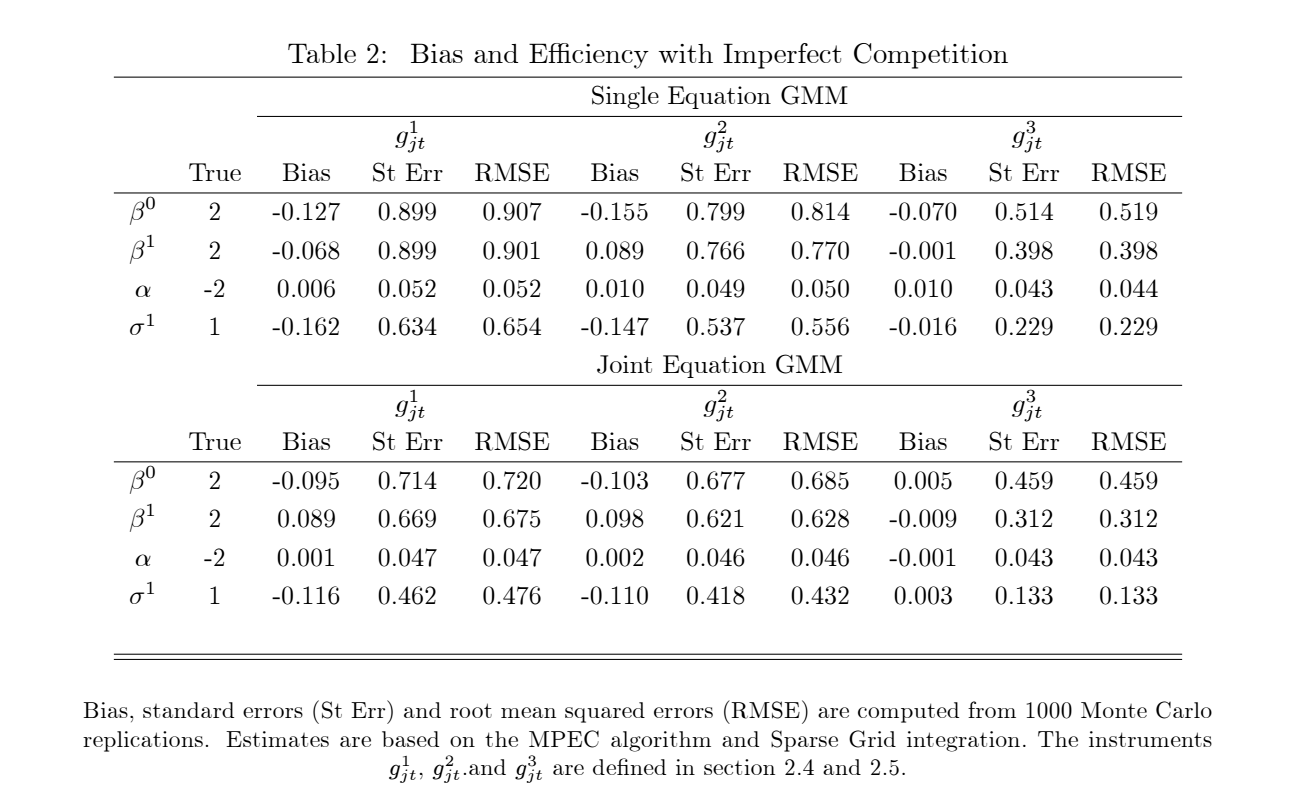
\includegraphics[width=4in]{resources/verboven.png}
\end{center}
\end{frame}


\begin{frame}{Differentiation Instruments: Gandhi Houde (2016)}
\begin{center}
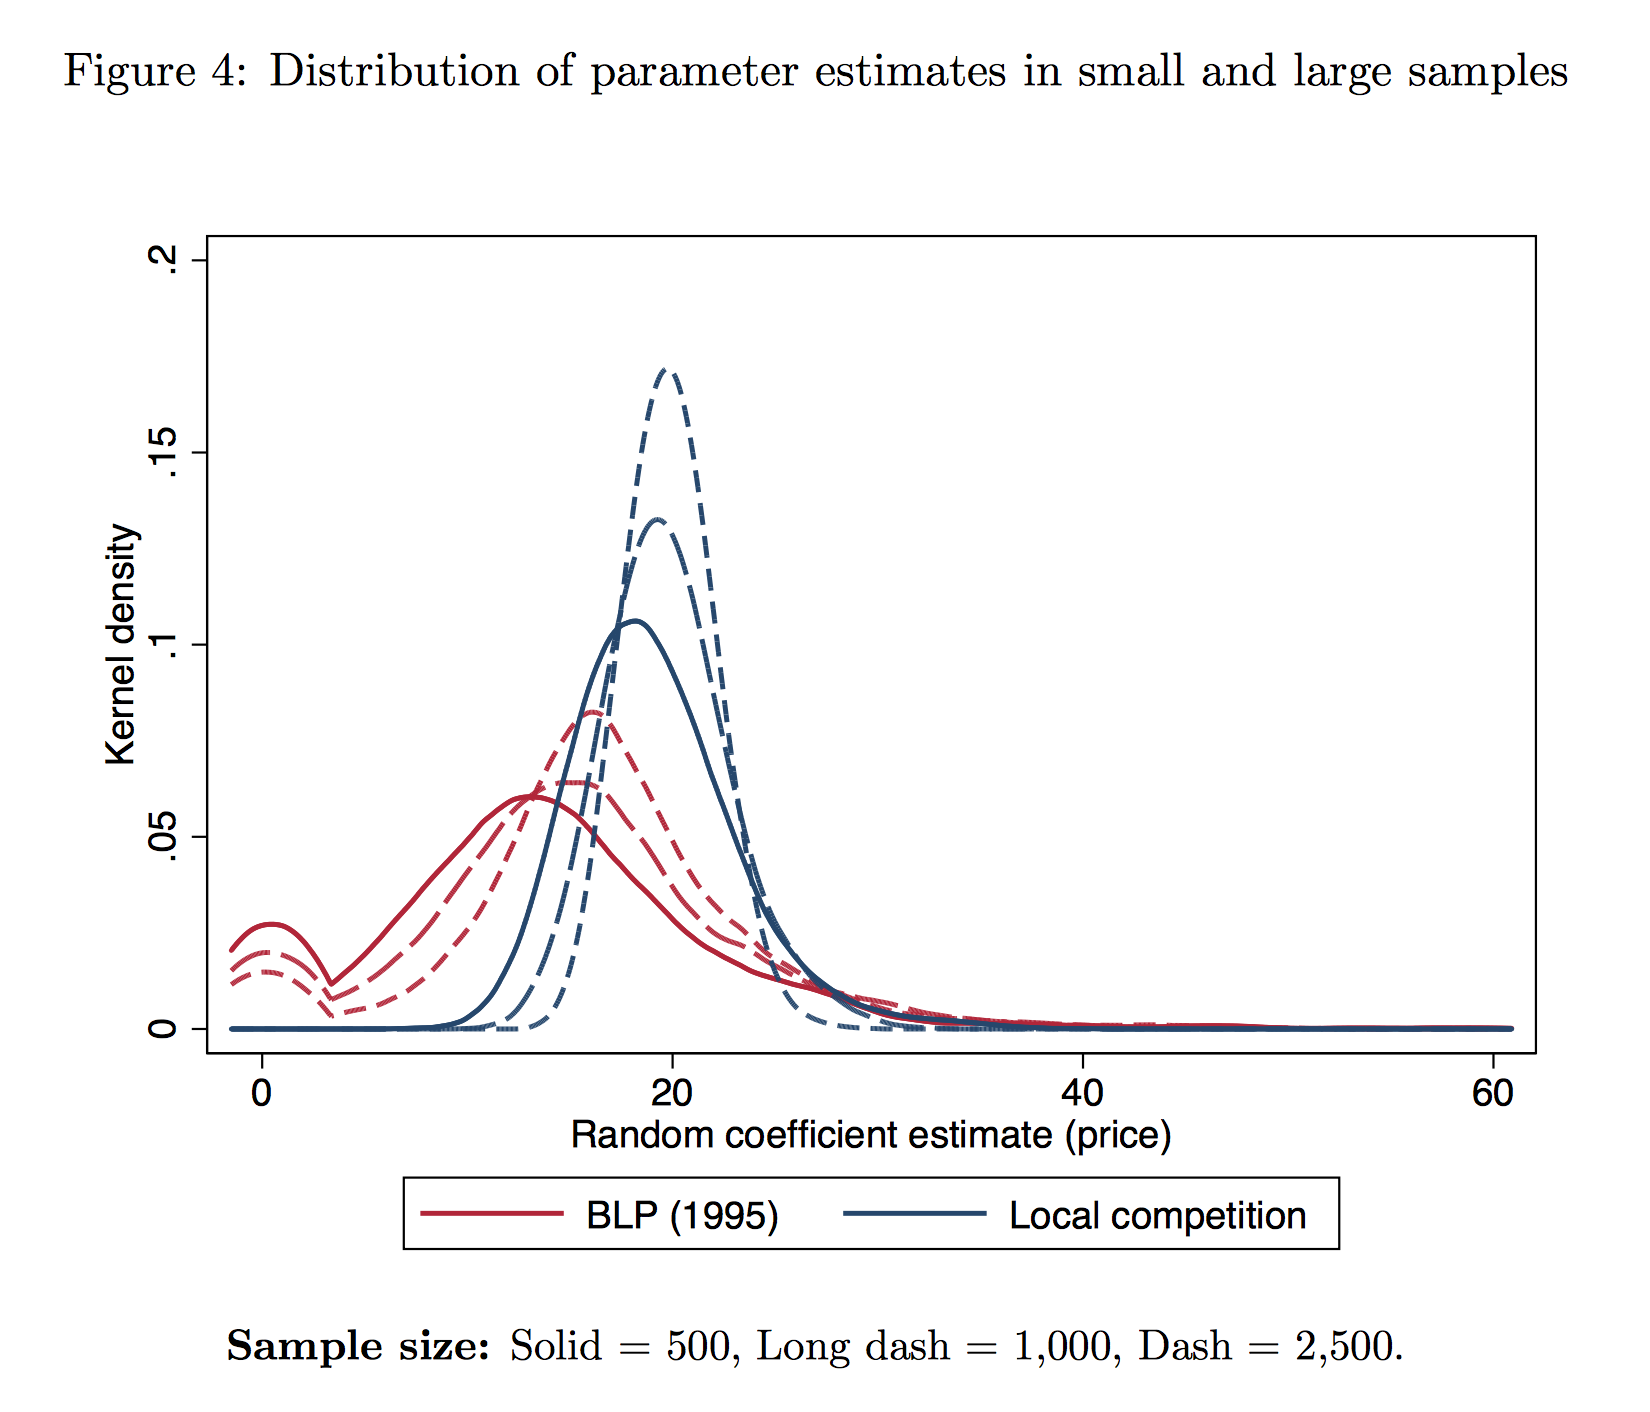
\includegraphics[width=3.8in]{resources/d_iv1.png}
\end{center}
\end{frame}

\begin{frame}{IV Comparison: Conlon and Gortmaker (2019)}
\begin{center}
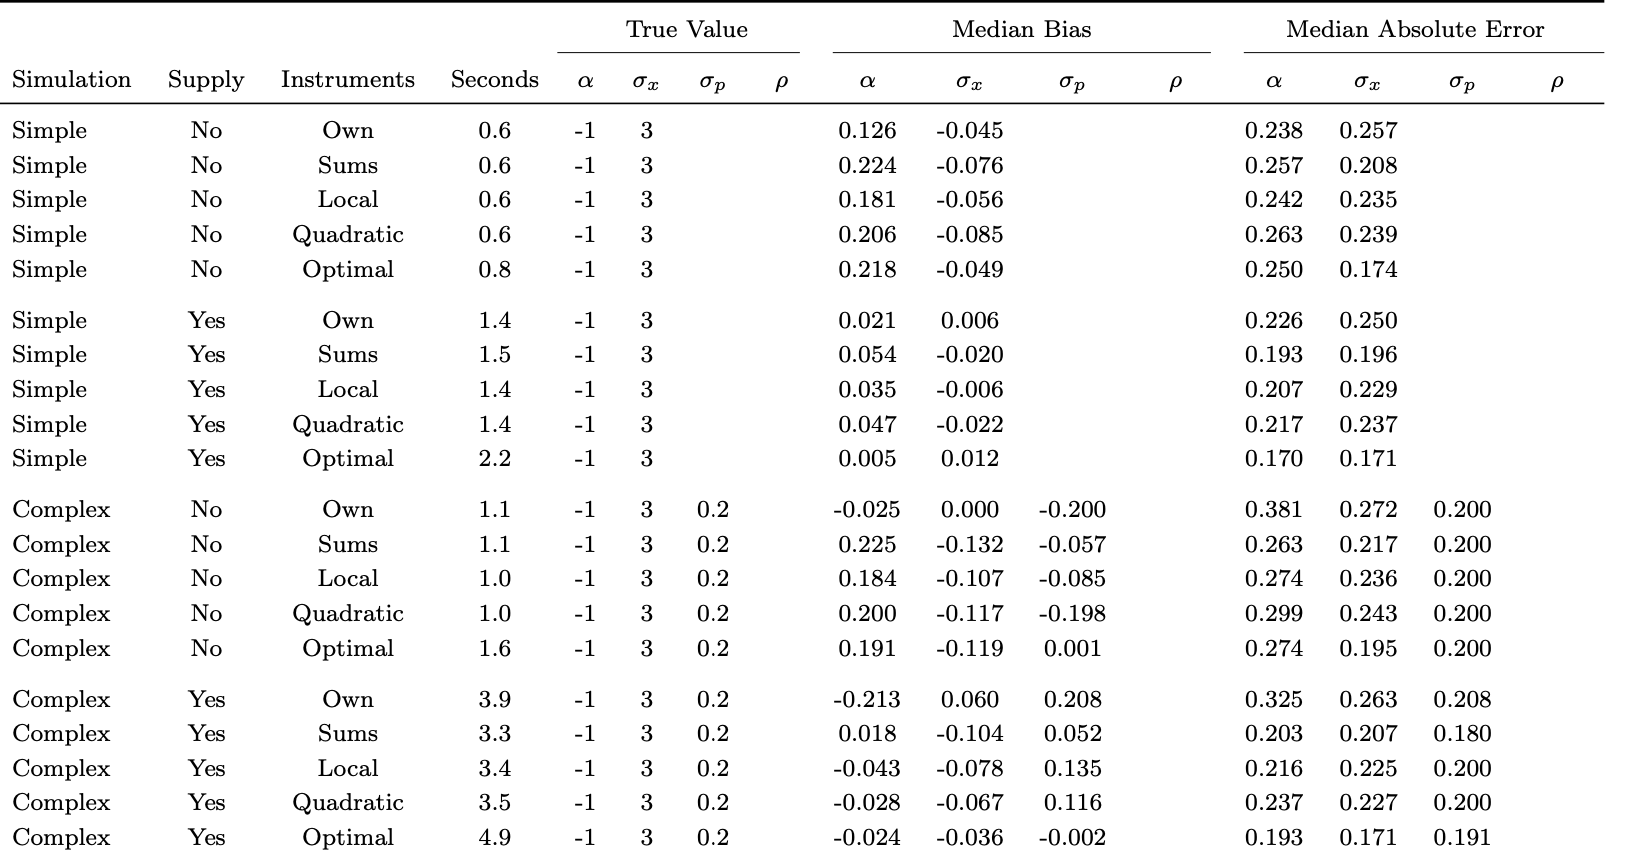
\includegraphics[width=4.9in]{resources/inst_table.png}
\end{center}
\end{frame}

\begin{frame}{IV Comparison: Conlon and Gortmaker (2019)}
\begin{center}
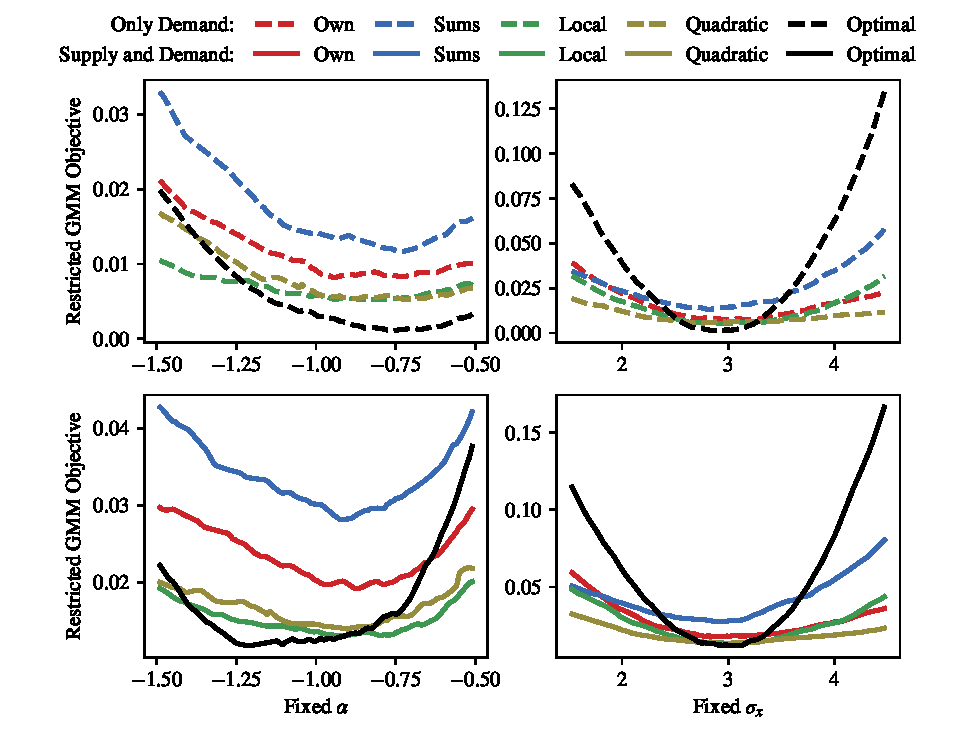
\includegraphics[width=3.9in]{resources/fixed_parameters_simple_plot.pdf}
\end{center}
\end{frame}




%
%
% \begin{frame}
%\frametitle{BLP Alternatives}
%\begin{itemize}
% \item BLP give us both a statistical \alert{estimator} and an \alert{algorithm} to obtain estimates.
%\item Plenty of other algorithms exist
%\begin{itemize}
%\item We could solve for $\delta$ using the contraction mapping, using \texttt{fsolve} / Newton's Method / Guess and Check (not a good idea!).
%\item We could try and consider a non-nested estimator for the BLP problem instead of solving for $\delta(\theta),\xi(\theta)$ we could let $\delta,\xi,\alpha,\beta$ be free parameters.
% \end{itemize}
%\item We could think about different statistical estimators such as $K$-step GMM, Continuously Updating GMM, etc.
% \end{itemize}
%\end{frame}
%
%
% \begin{frame}\frametitle{Dube Fox Su (2012)}
%\footnotesize
%\begin{eqnarray}
%\label{blpnfxp}
%\nonumber \arg \min_{\theta_2} && \psi' \Omega^{-1} \psi \quad \mbox{ s.t. } \\
%\nonumber \psi &=& \xi(\theta_2)' Z\\
%\xi_{jt}(\theta) &=& \delta_{jt}(\theta_2) - x_{jt} \beta - \alpha p_{jt} \\
%\nonumber \log(S_{jt})  &=& \log(s_{jt}(\delta,\theta_2))
%\end{eqnarray}
%
%\begin{eqnarray}
%\label{blpmpec}
%\nonumber \arg \min_{\theta_2,\alpha,\beta, \xi,\psi} && \psi' \Omega^{-1}  \psi \quad \mbox{ s.t. } \\
% \psi &=& \xi' Z\\
%\nonumber \xi_{jt} &=& \delta_{jt} - x_{jt} \beta - \alpha p_{jt} \\
%\nonumber \log(S_{jt})  &=& \log(s_{jt}(\theta_2, \delta))
%\end{eqnarray}
%\end{frame}
%
%\begin{frame}
%\frametitle{Comparing Approaches}
%\begin{itemize}
%\item The original BLP paper and the DFS paper define different \alert{algorithms} to produce the same statistical \alert{estimator}.
%\begin{itemize}
%\item The BLP algorithm is a \alert{nested fixed point} (NFP) algorithm. 
%\item The DFS algorithm is a \alert{mathematical program with equilibrium constraints} (MPEC).
%\item The unknown parameters satisfy the same set of first-order conditions. (Not only asymptotically, but in finite sample).
%\item $\hat{\theta}_{NFP} \approx \hat{\theta}_{MPEC}$ but for numerical differences in the optimization routine.
%\end{itemize}
%\item Our choice of algorithm should mostly be about computational convenience.
%\end{itemize}
%\end{frame}
%
%\begin{frame}
%\frametitle{BLP: NFP Advantages/Disadvantages}
%\begin{itemize}
%\item Advantages
%\begin{itemize}
%\item Concentrate out all of the linear in utility parameters $(\xi,\delta,\beta)$ so that we only search over $\Sigma$. When $\dim(\Sigma)=K$ is small (few dimensions of unobserved heterogeneity) this is a big advantage. For $K \leq 3$ this is my preferred approach.
%\item When $T$ (number of markets/periods) is large then you can exploit solving in parallel for $\delta$ market by market.
%\end{itemize}
%\item Disadvantages
%\begin{itemize}
%\item Small numerical errors in contraction can be amplified in the outer loop, $\rightarrow$ tolerance needs to be very tight.
%\item Errors in numerical integration can also be amplified in the outer loop $\rightarrow$ must use a large number of draws/nodes.
%\item Hardest part is working out the Jacobian via IFT.
%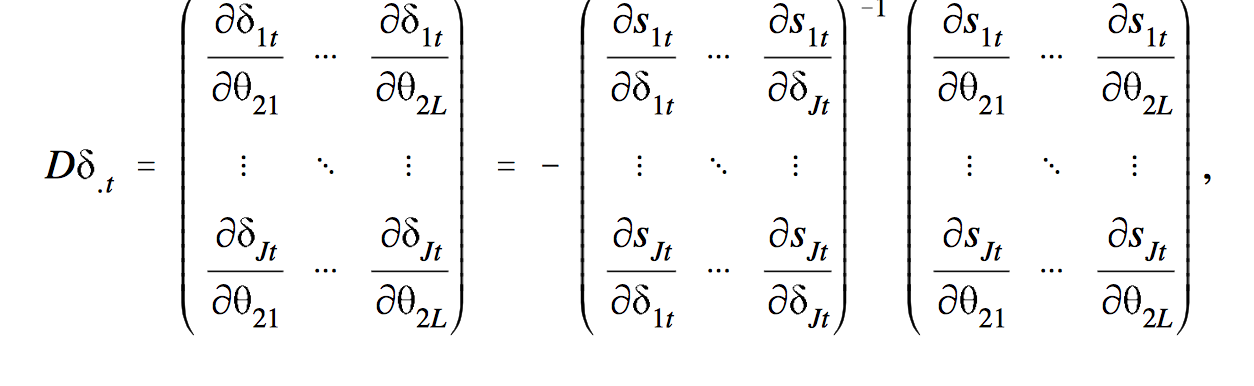
\includegraphics[width=2.8in]{resources/implicit_function.png}\\
%\end{itemize}
%\end{itemize}
%\end{frame}
%
%\begin{frame}
%\frametitle{BLP: MPEC Advantages/Disadvantages}
%\begin{itemize}
%\item Advantages
%\begin{itemize}
%\item Problem scales better in $\dim(\Sigma)$.
%\item Because all constraints hold at the optimum only: less impact of numerical error in tolerance or integration.
%\item Derivatives are less complicated than $\frac{\partial \delta}{\partial \theta}$ (no IFT).
%\end{itemize}
%\item Disadvantages
%\begin{itemize}
%\item We are no longer concentrating out parameters, so there are a lot more of them! Storing the (Hessian) matrix of second derivatives can be difficult on memory.
%\item We have to find the derivatives of the shares with respect to all of the parameters $\beta,\xi,\theta$. (The other derivatives are pretty easy).
%\item Parallelizing the derivatives is trickier than NFP case.
%\end{itemize}
%\end{itemize}
%\end{frame}


%
%\begin{frame}{Differentiation Instruments: Gandhi Houde (2016)}
%\begin{center}
%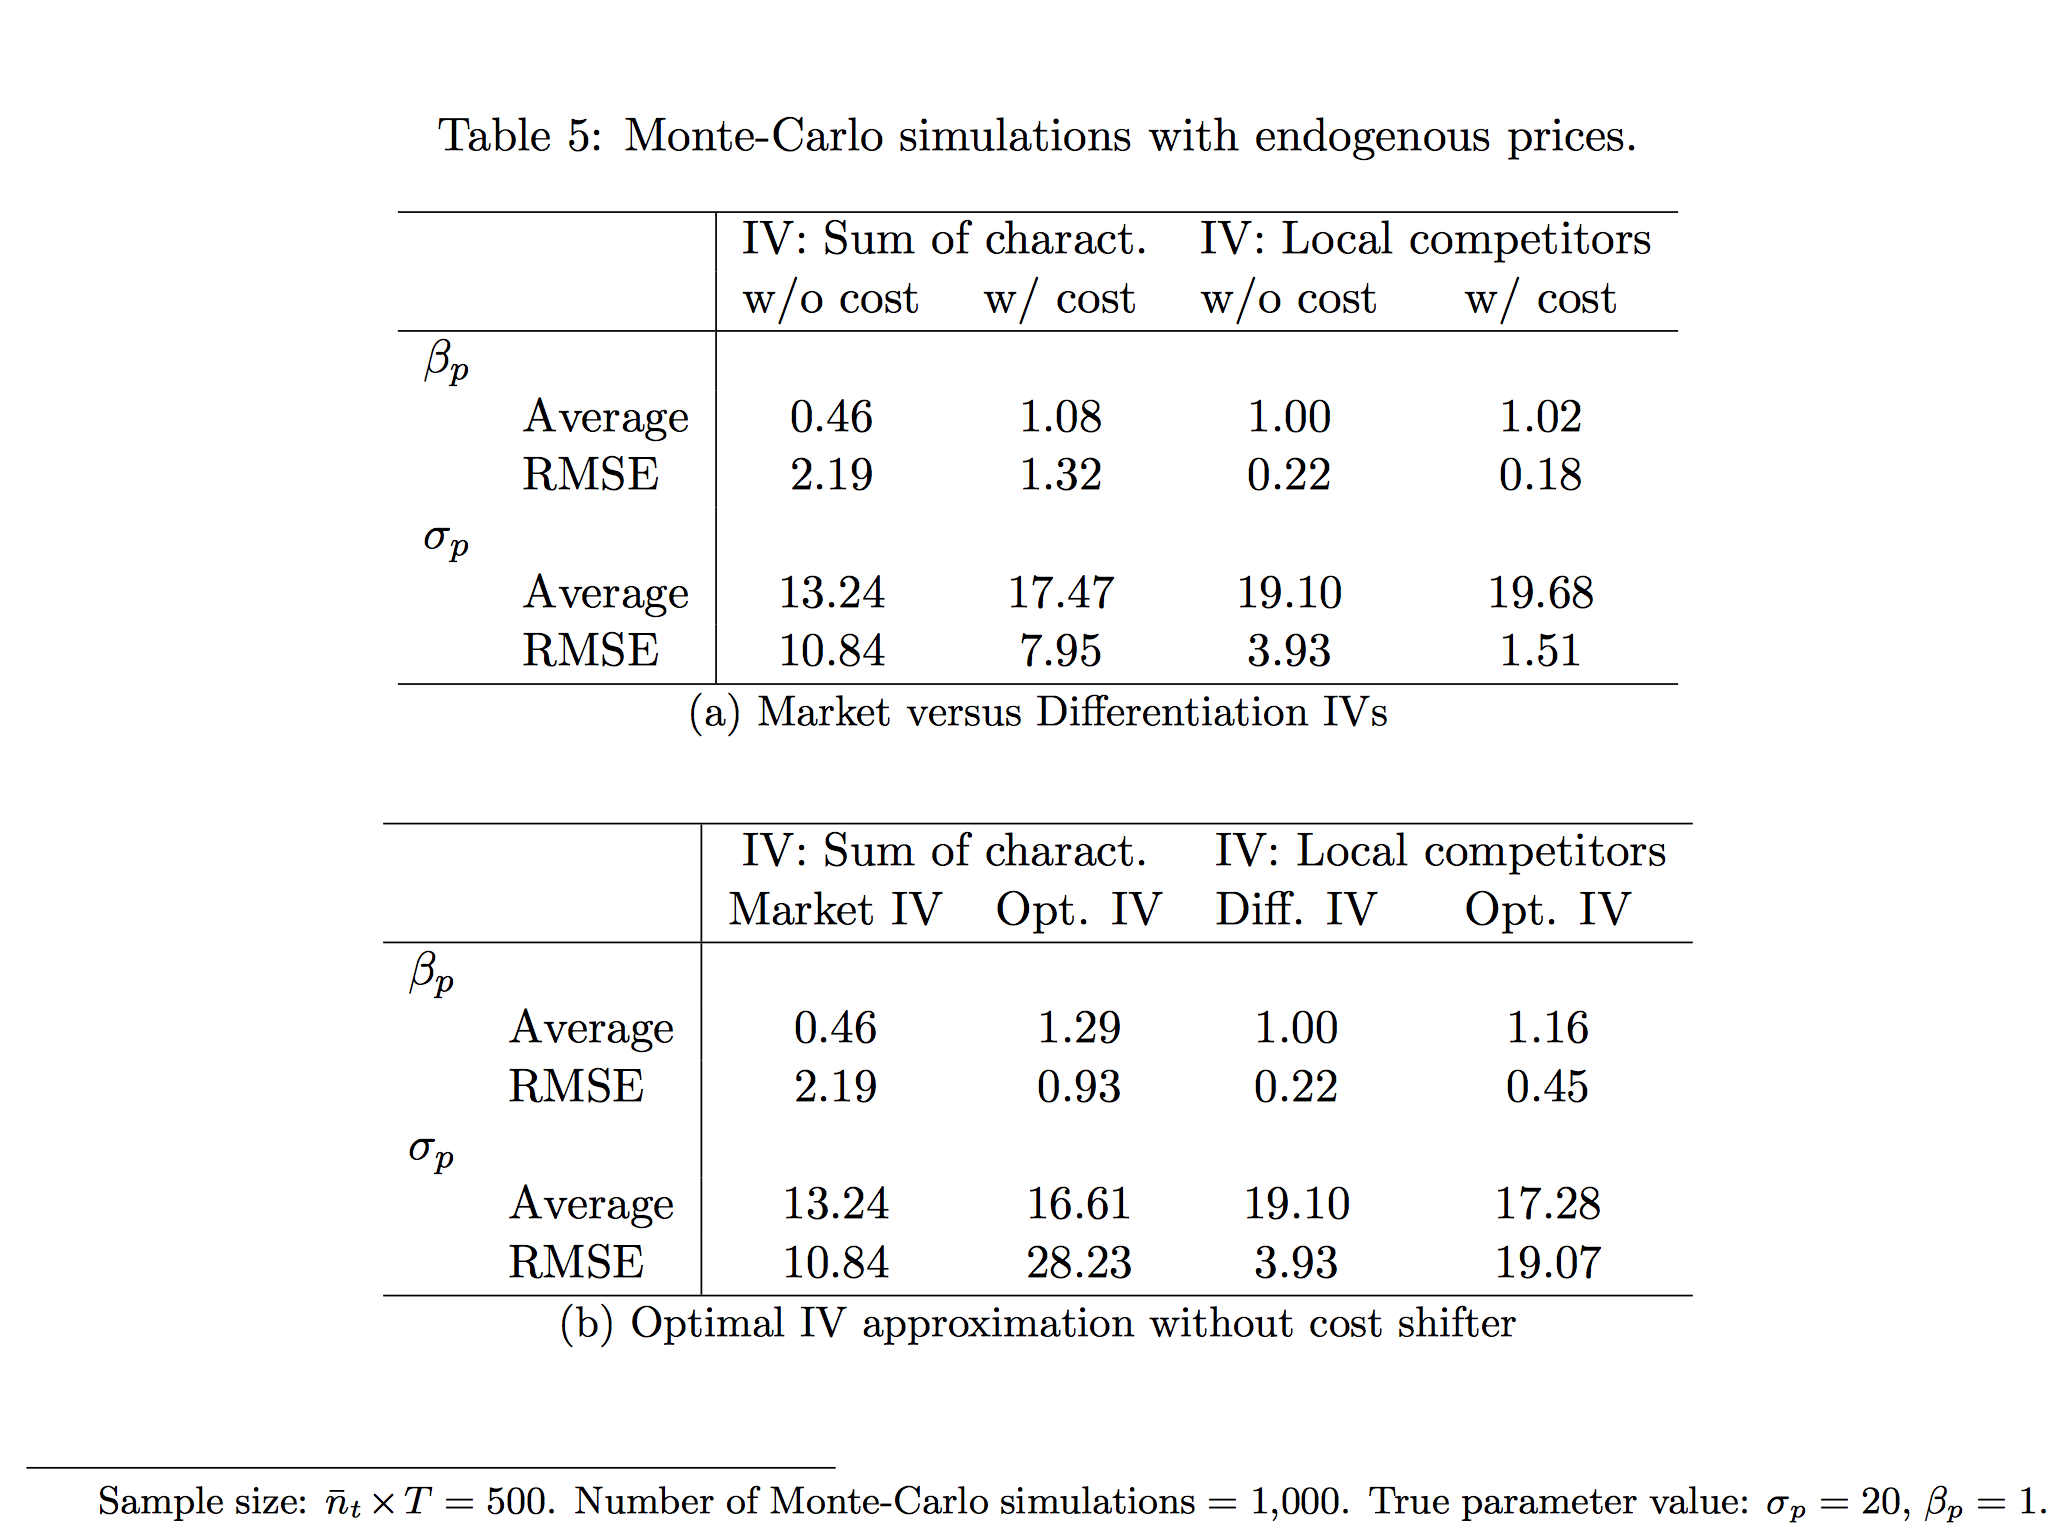
\includegraphics[width=3.8in]{resources/d_iv2.png}
%\end{center}
%\end{frame}
%

 

%
%\begin{frame} \frametitle{Extensions: Supply Moments}
%\begin{itemize}
%\item We can also impose the Bertrand FOC as a set of additional moments.
%\item First parametrize marginal cost
%\begin{eqnarray*}
%\ln mc_{jt} = \gamma_1 x_{jt} + \gamma_2 w_{jt} + \omega_{jt}
%\end{eqnarray*}
%\item helpful to constrain MC to be positive always.
%\item Note that for any vector of prices $p$ and demand parameters $\theta$ we can recover a unique vector of marginal costs (by solving the system of linear equations).
%\item Imposing the supply side only helps if we have information about the marginal costs / production function that we would like to impose
%\item Imposing these restrictions is helpful in constraining markups (so that implied MC are always positive, etc.).
%\item Misspecified functional forms for costs can cause problems!
%\end{itemize}
%\end{frame}





\end{document}